\chapter{可解释性}
\label{chap:trust-interpretability}

一封邮件被模型拦截后，解释可能服务于三种问题：用户询问哪些内容触发判断，开发者排查模型是否使用了不稳定页脚，受影响者寻找恢复业务的行动。第一种固定一次输出，第三种要求可行补救；第二种需先指定邮件范围与依赖指标，也可以从单次误拦提出假设，再在总体样本中检验。解释的证据要随问题确定，特征热力图不能自动覆盖这些用途。

按第~\ref{chap:trust-foundations}章的三层架构，可解释性主要提供证据能力，支持理解、质疑与补救。属性或规范层先确定需要解释的行为和用途，生命周期层再检查解释可以向谁公开、版本变化后是否有效以及有意规避下能否保持。解释本身也因此需要明确使用条件。

\term{可解释性}（interpretability）研究人能否通过适当表示与证据理解模型行为。第~\ref{chap:trust-robustness}章用模板变化暴露捷径，前一章评价行为并设置约束，这里进一步定位行为依据。一次失效测试只能提出解释问题，还需相应方法核验。本章先区分目的与范围，再介绍整体和单次解释、质量检查及行动补救；第~\ref{chap:trust-reliability}章的预测可靠性为这些解释提供相关但不同的证据。

\section{模型的可解释性}
\label{sec:interpretability-purpose}

\subsection{解释对象决定证据}

解释首先应说明解释什么、交给谁，以及支持什么判断。开发者可能需要内部激活和训练样本，普通使用者可能只需相关因素及适用限制，寻求补救的人则需要行动条件。信息的粒度应与任务匹配，不能按数量多少判断解释是否有用。

模型行为、计算机制与现实因果关系也需分开。年龄与输出相关是行为描述；在模型输入中修改年龄，可以检验模型如何使用字段；现实中改变年龄通常无法作为行动，更无法由字段试验推出后果。使用“影响”时，应指出比较的对象和干预发生在哪个系统中。

\subsection{整体解释与单次解释}
\label{sec:interpretability-global-local}

\term{整体解释}（global explanation）以可理解形式概括明确输入集合或参考分布上的判断规律，例如可执行规则、特征响应曲线和概念作用统计。整体指声明的覆盖范围，可能是全部部署邮件，也可能是某种语言或业务类型。它不要求逐项列出内部计算，但平均摘要不能因此被推广到每个输入。

\term{单次解释}（local explanation，常译“局部解释”）固定一项输出，例如当前邮件的拦截结果。方法可以比较输入邻域、相对基准的分数差或某次运行中的计算作用，几何邻域只是可能的选择。两类解释都需要可核查证据；整体主张要交代总体覆盖，单次主张则要固定参照、邻域或运行条件。

准确的整体加性规则可通过代入当前特征解释一次预测；多次归因也可在定义固定后汇总为总体摘要。反向作用的子群可能在均值中抵消，单个案例也不能支持普遍规律。整体或单次范围与参数访问条件是独立维度，输入输出查询可以用于两者。

\begin{example}[同一规则的整体与单次说明]
\label{ex:interpretability-global-local}
设教学邮件评分器使用二元特征$x_1$和$x_2$，分别表示支付要求与可执行附件，规则为$f(x_1,x_2)=1+2x_1+4x_2$，分数至少为6时隔离。这里分数并非概率。整体说明给出基准、两项增量和阈值，覆盖四种组合；当前$(1,1)$的单次说明则代入得到$1+2+4=7$，相对$(0,0)$贡献为2和4。代入解释了本次计算，要断言真实模型的整体规则还须取得结构或查询证据。
\end{example}

图~\ref{fig:trust-global-local-explanation}分别展示规则范围和单次代入。左侧覆盖四种输入，右侧只固定当前组合，两者承担不同的核验任务。

\begin{figure*}[htbp]
  \centering
  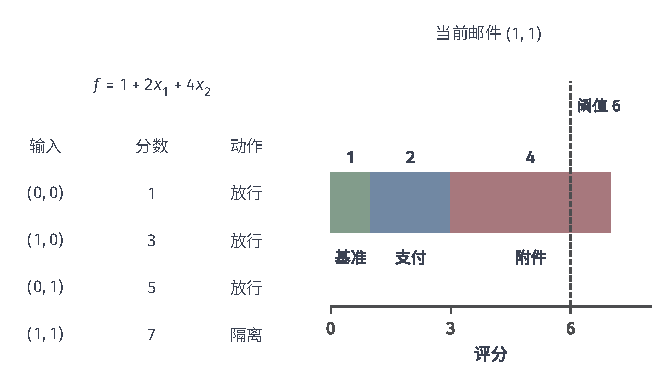
\includegraphics[width=113.404mm]{figures/03-foundations/03-trustworthiness/tikz/trust-global-local-explanation/figure.pdf}
  \caption{示例~\ref{ex:interpretability-global-local}的规则覆盖与代入。左侧列出四种组合的规则，右侧对$(1,1)$计算基准1加贡献2、4，得到7并与阈值6比较。计算分数不作概率解释，特征贡献也未表达现实因果作用；单次代入与整体覆盖分别需要核验。}
  \label{fig:trust-global-local-explanation}
\end{figure*}

\subsection{解释的表示与证据条件}

结构易于追踪还要求特征含义明确。稀疏线性式或短规则表若操作的是上万个未命名嵌入维度，使用者仍难以理解。复杂模型的局部行为也可能由简单规则准确近似，但近似范围需要限制在已验证区域。

可用信息决定能够提出的证据：输入输出查询支持行为近似，参数与激活访问支持机制假设，重新训练则支持更直接的数据影响检验。阅读后续方法时，应先核对所需访问条件，再判断它能回答的问题。

解释还隐含参照。当前邮件为何被拦而相似邮件没有，是输入比较；为何隔离而非人工复核，是行动比较。两种问题需要不同背景、分数与约束，同一归因算法也会随基准改变答案。交付时应列明输出、接收者、支持的判断或行动、参照、输入范围及允许变化的因素。

\section{整体行为的解释}
\label{sec:interpretability-global}

整体解释可围绕计算结构、输入作用和语义概念展开。结构交代规则如何组合输出，输入分析检查可观察因素的变化，语义分析检验这些因素对应的概念。三方面可以结合，例如可读结构通过命名概念计算；以下分类依据主要解释对象，不把它们当成互斥模型类型。

\subsection{基于模型结构的解释}
\label{sec:interpretability-global-response}

解释整套计算规则有两条途径：使用可读的实际预测器，或在训练后拟合可读代理。前者需要验证任务表现和结构理解，后者除可理解性外，还需检验与原模型的符合程度。规则来自哪个模型应在解释中明确。

\term{广义加性模型}（generalized additive model, GAM）把预测分解为单特征函数，以便逐项查看：
\begin{equation}
 f(\bm{x})=\beta_0+\sum_{j=1}^{d}f_j(x_j)\, .
 \label{eq:interpretability-gam}
\end{equation}
$\beta_0$为基准，$f_j$描述第$j$项特征响应；回归时$f$可直接作为预测，二分类时可作为对数几率并经逻辑函数转为概率。各函数需固定中心化约定，例如训练分布均值为零。曲线斜率表示模型敏感性，样本覆盖则帮助区分有数据支持和估计不稳的区域\scite{hastie1986gam}。

相加结构不能表示所有交互。例如，支付要求与附件各自出现可能正常，共同出现才改变风险判断。Lou等在单变量项之外加入少量$f_{j,k}(x_j,x_k)$，用二维曲面表示条件作用。训练需要选择交互并控制复杂度，解释也应同时展示单项曲线和交互曲面\scite{lou2013ga2m}。

树与规则同样可以追踪路径，但数量、重复条件和深度会增加阅读负担，只展示常见路径还会遗漏低频分支。应在具体任务中同时比较预测损失与使用者的判断表现，再确定可读结构是否足够。模型复杂程度本身不能替代这种比较。

实际预测器使用真实标签，在加性、平滑性或深度等结构限制下训练。训练固定后，解释展示函数、阈值和交互怎样组合输出。可理解性来自能够追踪的规则及特征，不能仅由训练方法名称判断。

已训练复杂模型可在声明分布上建立\term{整体代理}（global surrogate）。从该范围抽取输入，查询原模型$f$，再用其分数拟合可读模型族$G$中的浅树、规则或加性模型。令$\Omega$惩罚复杂度，$\lambda\geq0$控制权衡，一种目标为
\begin{equation}
 \hat g=\argmin_{g\in G}\left\{
 \frac1n\sum_{i=1}^n\bigl[f(\bm{x}_i)-g(\bm{x}_i)\bigr]^2
 +\lambda\Omega(g)\right\}\, .
 \label{eq:interpretability-global-surrogate}
\end{equation}
拟合对象是$f(\bm x_i)$，所以用真实标签$y_i$另训小模型并不自动形成解释。分类代理可以拟合概率或类别，所选目标决定保留的是分数变化还是决策边界。

代理应交付实际规则，并在另留查询样本上比较$g$与$f$。示例~\ref{ex:interpretability-global-local}的教学规则可由先看附件、再看支付要求的树复述；“有附件就隔离”却会在$(0,1)$上出错。整体平均一致率达到预设阈值后，也须检查关键业务分支；可提高复杂度或收窄范围，但同时报告增加的理解负担。

\subsection{基于输入的解释}
\label{sec:interpretability-global-dependence}

代理给出可重新计算的近似规则，输入摘要则只回答特定作用问题。可以研究特征变化时分数如何响应，也可以破坏信息后比较任务损失。前者描述函数形状，后者描述固定模型对该信息的性能依赖，所需标签与判断尺度不同。

\paragraph{响应形状与交互}

\term{部分依赖}（partial dependence, PD）把目标特征固定，对其他特征取平均\scite{friedman2001gradientboost}。设输入参考分布为$P_{\mathrm{ref}}$，$\bm X\sim P_{\mathrm{ref}}$，对其支持范围中的$t$定义
\[
 \operatorname{PD}_j(t)
 =\mathbb E_{\bm X_{-j}\sim P_{\mathrm{ref},-j}}
 f(t,\bm X_{-j})\, .
\]
$\bm X_{-j}$为其他特征，$P_{\mathrm{ref},-j}$为相应边缘分布。这个定义固定了被替换字段和平均总体，曲线应随这两项条件解读。

经验曲线从参考总体采样，在每个$t$处把所有样本第$j$项替换后查询模型，计算
\[
 \widehat{\operatorname{PD}}_j(t)
 =\frac1n\sum_{i=1}^n f(t,\bm{x}_{i,-j})\, .
\]
将均值按$t$排列可显示阈值、单调性或饱和。两特征分析可在二维网格重复操作，检查交互；平均之外还应查看个体曲线，以识别方向不同的响应。

示例~\ref{ex:interpretability-global-local}的四种组合等概率时，$\operatorname{PD}_1(t)=3+2t$、$\operatorname{PD}_2(t)=2+4t$。这给出平均分数响应，未给出每封邮件的预测，也未使用真实标签检验正确性。参考群体改变可以改变截距；本例没有交互，斜率仍为2和4。

替换可能使输入离开观测支持。若数据恒满足$x_1=x_2$，模型$f(x_1,x_2)=x_1-x_2$在观测上总为零，单独改变$x_1$仍会得到上升曲线。该曲线描述人工组合上的模型响应，不能作为观测人群中的现实效应。

按目标特征条件化其他特征，可减少部分无效组合，同时会把特征关联纳入平均。因而应明确使用边缘还是条件分布，不能仅从同样形状的曲线推断它们解释的是同一作用。

\term{累积局部效应}（accumulated local effects, ALE）在现有取值附近估计小幅变化，再沿特征累积，以减少远离数据支持的替换。对适当光滑模型，一阶定义为
\begin{equation}
 \operatorname{ALE}_j(t)
 =\int_{t_0}^{t}
 \mathbb E_{P_{\mathrm{ref}}}\!\left[
 \frac{\partial f(s,\bm X_{-j})}{\partial s}
 \,\middle|\,X_j=s\right]\mathrm ds-C_j\, ,
 \label{eq:interpretability-ale}
\end{equation}
$t_0$是积分起点，$C_j$使结果在同一$P_{\mathrm{ref}}$下中心化。实际可将取值分箱，在每箱已有样本上查询边界差并累加平均差，不必计算导数\scite{apley2020ale}。

PD平均完整输出，ALE平均局部变化。ALE减少部分外推，但粗分箱可能越过无数据区，细分箱又可能缺少样本；模型在数据流形外的延伸仍可能影响局部导数。这些方法未识别现实因果作用。保留个体响应曲线可进一步检查总体均值遗漏的交互。

\paragraph{任务表现对信息的依赖}

曲线没有利用真实结果，因而不能说明敏感性是否有助于分类。检查模型是否靠页脚正确判断，需要对同一模型比较保留和破坏页脚信息时的损失。这个问题以任务表现为依据，不能由系数大小回答。

\term{置换重要性}（permutation importance）固定模型，打乱测试样本中某字段并比较损失。应在同一批样本上成对计算，重复置换，报告增量及波动\scite{breiman2001randomforests,strobl2007bias}。超过预设阈值的损失增量支持该破坏规则下的性能依赖，依赖是否合理或是否具有现实因果意义仍需其他判断。

设$\pi$为样本索引排列，$\bm x_i^{(j,\pi)}$仅将第$j$项替换为$x_{\pi(i),j}$，一次置换的损失增量是
\begin{equation}
 \widehat I_j^{(\pi)}
 =\frac1n\sum_{i=1}^n\left[
 \ell\bigl(f(\bm{x}_i^{(j,\pi)}),y_i\bigr)
 -\ell\bigl(f(\bm{x}_i),y_i\bigr)\right]\, .
 \label{eq:interpretability-permutation}
\end{equation}
$y_i$用于比较任务损失，模型全程不重训练。教学测试100封邮件，误判由10增至25，增量为0.15。重复试验反映置换随机性，推广到新邮件总体时还应考虑测试样本不确定性。

页脚与发送方配套时，单独置换会制造无效组合，使损失混入分布外效应。按发送方分组置换研究剩余信息，联合置换研究整组信息。互相替代的字段中，模型未使用的那一项可有零重要性，但仍包含预测信息；删除后重训练则检验学习系统能否利用替代信息，应单独报告。

响应与性能依赖可以不同。分数变化未跨分类阈值时，零一损失增量可能很小；破坏被错误使用的信息甚至会降低损失。曲线描述模型怎样响应，置换损失描述响应对所选指标的后果，任务语义再决定该依赖能否接受。

\subsection{基于语义的解释}
\label{sec:interpretability-global-concepts}

输入字段未必对应读者关心的含义。“催促付款”有多种表达，同一词也可能属于引用或警示。语义解释以来源可验证、立即转账等概念组织证据，可以把概念放进实际预测路径，也可以在已有表示中检验概念方向。

Koh等的\term{概念瓶颈模型}（concept bottleneck model）先预测人定义的概念，再只通过概念判断结果。语义接口因而进入模型计算，可以查看和修改；它区别于输出后附加概念描述\scite{koh2020conceptbottleneck}。

设概念$\bm c\in\mathbb R^m$、概念预测器$g$与决策函数$h$，则$f(\bm x)=h(g(\bm x))$。有概念标签时，可以先训练$g$再用真实或预测概念训练$h$，也可以联合任务和概念损失。不同训练方式决定任务信号是否改变概念，以及使用时的概念误差是否与训练一致。人工确认邮件来源后，可替换对应概念并重新检查输出。

整套规则解释仍须说明$h$怎样组合概念，例如给出加性项、阈值或路径。复杂$h$提供可核查接口，却没有自动展开全部计算。要概括概念作用，应在目标任务样本中检验，而非仅展示一次成功纠正。

命名接口仍可能出错：概念误判向下游传播，概念遗漏降低任务能力，连续分数还可能携带名称之外的信息。若存在绕过瓶颈的路径，概念替换也不能控制所有依据。验收应共同核查概念质量、替换效果与任务损失。

\term{概念激活向量检验}（testing with concept activation vectors, TCAV）在已有表示中提出语义假设。Kim等用概念与对照样本在某层训练线性分隔器，得到朝目标概念的方向$\bm v_C$，再统计类别分数沿该方向导数为正的比例。它把模型对概念的使用问题转为可重复的表示敏感性检验，无须重训概念瓶颈\scite{kim2018tcav}。

若激活为$\bm h(\bm x)$、后续类别分数为$s_k(\bm h)$，被统计的是$\nabla_{\bm h}s_k(\bm h(\bm x))^\top\bm v_C$的符号。样本、对照与层都影响结果，应重复拟合并报告不确定性。可分方向可能捕捉共现背景，正导数也只是内部局部敏感性；它既非现实概念干预的概率效果，也未限制模型只能使用所命名概念。

实施时，概念实例与对照用于学习方向，目标任务样本用于测作用，另留样本用于复核。固定模型和层后，记录激活、训练线性分类器、确定正类朝向，再计算各目标样本方向导数。对集合$\bm D_k$，可汇总为
\[
 \widehat t_{C,k}
 =\frac1{|\bm D_k|}\sum_{\bm{x}\in\bm D_k}
 \mathbb I\!\left\{
 \nabla_{\bm h}s_k(\bm h(\bm{x}))^\top\bm v_C>0
 \right\}\, .
\]
100个样本中80个正导数对应0.8，表示八成样本有正局部敏感性，不能读为贡献占80\%。更换概念实例和随机对照后，若目标方向持续高于随机方向，并报告差值与不确定性，才加强概念假设的证据。

结构、输入与语义各自解释组合方式、字段作用及对应含义。概念瓶颈改变实际结构，TCAV检验已有表示，因此同一方法可以连接多个方面。整体结论还须交代样本覆盖、汇总规则及方向相反的子群。

\section{单次行为的解释}
\label{sec:interpretability-local}

单次行为可追溯到输入、运行计算和训练经历。误拦邮件的三个问题分别是哪些内容触发、哪些组件参与处理，以及哪些学习样本使模型形成这种判断。解释范围固定在当前行为，但各方法改变的对象不同。

相似案例、反事实、代理与归因都固定训练结果并分析输入响应。内部解释检查当前计算作用，数据解释则改变学习经历并观察同一输入的结果。以下按论断对象组织方法，输入查询或参数访问只规定获得证据的条件。

解释前应指定输出是垃圾邮件分数、隔离动作还是隔离与复核之间的选择。阈值和权限也参与最终动作，只解释分数可能遗漏它们。下文以$f(\bm x)$表示目标标量分数，$\hat y(\bm x)$表示经决策规则得到的类别或动作；多类别时还须固定类别。

\subsection{基于推理输入的解释}
\label{sec:interpretability-local-input}

输入解释通过检索参照或构造变化，把当前结果与输入差异联系起来。同结果近邻提示共同因素，不同结果近邻提示边界，系统变化则可拟合响应或分配贡献。方法的共同对象是固定模型的输入输出，交付的证据形式不同。

输入分析可以检索原有样本，也可以读取导数，不一定实际修改当前邮件。最终类别相同仍可能伴随超过预设幅度的分数变化，因此应记录究竟比较分数、类别还是动作。

\paragraph{相似案例的对照}
\phantomsection
\label{sec:interpretability-local-examples}

\term{基于案例的解释}（example-based explanation）展示与当前输入相似且判断相同的参照。例如，支付要求与可执行附件触发隔离时，可显示同样包含两项因素的已隔离邮件，标记共同片段，让读者了解本次结果所在的案例组。

检索先要定义相似性采用词语、业务字段还是表示，以及可忽略的差异，再在参考库中显示近邻的距离、共同点和区别。有真实标签时应同时展示标签与预测，避免把相似误判当成正确依据。多个近邻或代表性原型可减少偶然选择的影响。

案例对照的证据强度取决于预测机制。近邻或原型模型可以显示实际参与的案例和权重；预测后再检索的案例只提供线索。若声称共同因素解释当前判断，还需改变这些因素并核对输出。

Chen等的原型部件网络（prototypical part network, ProtoPNet）比较图像局部与学习原型的表示相似度，再加权得到类别分数。原型关联训练片段，可以显示当前区域对应哪个典型部分及其分数作用。这里案例比较属于实际计算路径\scite{chen2019protopnet}。

相似性可能来自背景或邮件模板，与读者理解的物体和业务意图不同。应显示实际比较区域与贡献权重，减少读者自行猜测；相近而输出不同的案例还能帮助检查边界。

\paragraph{不同结果的反事实比较}
\phantomsection
\label{sec:interpretability-local-counterfactual}

反事实比较研究哪些差异能够改变当前判断。可检索真实的不同结果近邻，也可只修改少量条件重新查询。前者提供观察对照，后者通过控制其他因素检验变化作用。

Wachter等的\term{反事实解释}（counterfactual explanation）搜索接近当前输入而达到目标输出的候选，可优化距离与目标损失，也可把输出要求列为约束。方法将当前结果转换为明确的替代输入问题\scite{wachter2018counterfactual}。

设不同结果的目标集合为$Y_{\mathrm{target}}$，距离为$d$，有效输入集为$\bm X_{\mathrm{valid}}$，可求
\begin{equation}
 \min_{\bm{x}'\in\bm X_{\mathrm{valid}}}
 d(\bm{x}',\bm{x}),
 \qquad \hat y(\bm{x}')\in Y_{\mathrm{target}}\, .
 \label{eq:interpretability-counterfactual}
\end{equation}
搜索可从真实近邻、枚举或梯度方法开始，候选必须通过完整预测重新核验并列出改动。尺度、离散取值和有效组合应预先确定，否则最近可能只是单位选择的结果。有限搜索找到候选，也未证明最小性或唯一性。

沿用示例~\ref{ex:interpretability-global-local}，当前$(1,1)$得7分。将附件改为非可执行、保留支付要求后，$(1,0)$得3分；去掉支付要求、保留附件后，$(0,1)$得5分，两者均越过放行边界。因此，在另项不变时，任一改动都足够。只展示附件方案会遗漏另一条路径。

这些结论以固定模型、参照和允许改动为条件。多字段不同的真实近邻仅提示差异，受控重算进一步检验预测作用。预测变化还不说明现实因果后果或行动可行性；第~\ref{sec:interpretability-recourse}节将补上行动条件。

为了单独看清输入距离，图~\ref{fig:trust-counterfactual-nearest}改用示例~\ref{ex:interpretability-causal-recourse}中的连续申请场景。这里$s$为技能分数，$r$为当期资源，申请在$s+r\geq3$时批准。当前$(1,1)$到批准区域的欧氏最近点为$(1.5,1.5)$，这里只比较输入距离，尚未计算培训和支持的后果及成本。

\begin{figure}[!htb]
  \centering
  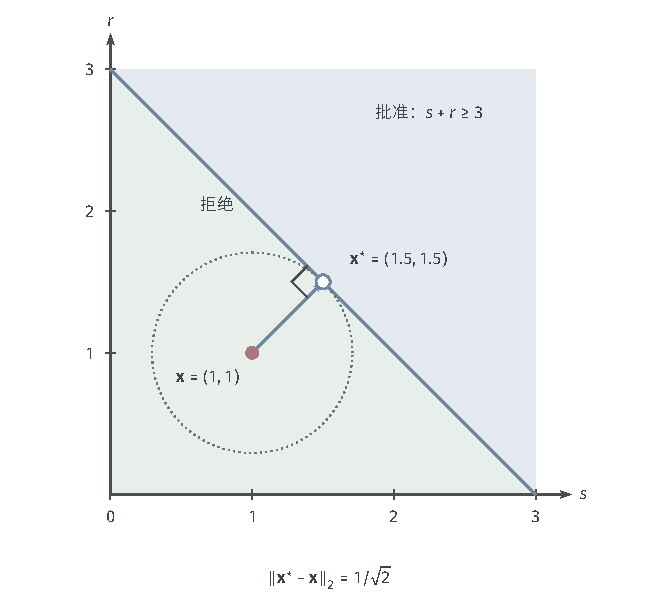
\includegraphics[width=\linewidth]{figures/03-foundations/03-trustworthiness/tikz/trust-counterfactual-nearest/figure.pdf}
  \caption{等权欧氏距离下的最近目标输入。从$(1,1)$到含边界$s+r=3$的批准区域，垂直投影为唯一最近点$(1.5,1.5)$，距离$1/\sqrt2$。虚线圆与直角记号分别显示等距和垂直关系。此处没有行动约束，实际补救路径另见图~\ref{fig:trust-actionable-recourse}。}
  \label{fig:trust-counterfactual-nearest}
\end{figure}

案例与反事实提供具体参照。若要系统说明当前分数，可拟合附近变化的响应规则，也可分配相对基准的差异。后面的代理、扰动与归因分别采用这些比较，输出数值应按所定义的问题解释。

\paragraph{附近输入的响应规则}
\phantomsection
\label{sec:interpretability-local-neighborhood}

\term{局部可解释模型无关解释}（local interpretable model-agnostic explanations, LIME）在当前输入附近查询模型，按接近程度加权拟合简单代理并惩罚复杂度。采样规则、距离与代理误差共同决定解释范围\scite{ribeiro2016lime}。

邮件词项保留向量$\bm z$可通过$r(\bm z)$映射成可查询文本。设代理族为$G$，接近权重为$w_{\bm x}$，复杂度为$\Omega$，$\lambda\geq0$，可拟合
\begin{equation}
 \hat g=\argmin_{g\in G}\left\{
 \sum_{i=1}^{n}w_{\bm x}(\bm{z}_i)
 \bigl[f(r(\bm{z}_i))-g(\bm{z}_i)\bigr]^2
 +\lambda\Omega(g)\right\}\, .
 \label{eq:interpretability-lime}
\end{equation}
把较大权重集中在较窄邻域，能突出当前输入，却减少可识别的变化；扩大高权重邻域，则可能超出简单模型的拟合能力。删词还可能破坏语法或任务目的，应核查邻域有效性并在另取邻域样本上报告误差。系数回答的是这个加权近似问题。

LIME的计算先采样可读的删词向量，查询原模型分数，再按距离拟合少量非零系数。解释交付所选词项、系数及邻域误差，原模型参数保持固定。这些对象共同说明代理在哪里、以多大误差近似当前响应。

示例~\ref{ex:interpretability-global-local}的加性规则若有足以识别两项作用的邻域样本，无稀疏惩罚的线性拟合可恢复2和4。存在交互时，词项系数可能随邮件改变。整体代理也采用查询后拟合，但其样本与误差覆盖总体，LIME则集中在当前输入的权重邻域。

邻域代理解释附近输入怎样改变输出，归因则标记当前证据或分配分数差。有的方法仅给出敏感位置，有的要求贡献之和满足规定差值。后一要求依赖基准与组合价值定义，数值应据此解读。

\paragraph{扰动比较与局部敏感性}

遮挡通过输入输出查询计算单项作用：按规定参照替换第$j$项，比较替换前后分数。文本可替换片段，图像可替换区域。交互与冗余会使各项移除效果不能相加为总差，替换规则也必须列入解释定义。

可微分$f$的梯度描述小幅输入变化的终点敏感性。饱和区的梯度可能很小，但该特征仍参与了较早的分数变化。若要分配相对基准的差异，需要规定路径并累计沿途作用。

\paragraph{相对于基准的贡献分配}
\phantomsection
\label{sec:interpretability-local-attribution}

\term{积分梯度}（integrated gradients, IG）选择基准$\bm x_0$并沿直线路径到$\bm x$积分各维导数：
\begin{equation}
 \operatorname{IG}_j(\bm{x})
 =(x_j-x_{0,j})\int_0^1
 \frac{\partial f(\bm{x}_0+t(\bm{x}-\bm{x}_0))}
      {\partial x_j}\,\mathrm dt\, .
 \label{eq:interpretability-ig}
\end{equation}
令$\bm\gamma(t)=\bm x_0+t(\bm x-\bm x_0)$、$\varphi(t)=f(\bm\gamma(t))$。若$\varphi$在$[0,1]$上绝对连续，各坐标的$(x_j-x_{0,j})\partial f(\bm\gamma(t))/\partial x_j$可积，并几乎处处满足
\[
 \varphi'(t)=
 \sum_j\frac{\partial f(\bm\gamma(t))}{\partial x_j}(x_j-x_{0,j})\, ,
\]
则积分链式关系与微积分基本定理给出$\sum_j\operatorname{IG}_j(\bm x)=f(\bm x)-f(\bm x_0)$。整条路径邻域连续可微是更强的充分条件。分段光滑模型也需检查复合函数和几乎处处链式关系；路径落在不可微集合且选用导数不代表路径导数时，不能直接援引完整性等式。

完整性表示相对基准的分数差得到分配，并未赋予基准或路径现实因果含义。Sundararajan等以归因公理提出该方法，空文本、黑图像或平均输入是否适合仍由任务决定\scite{sundararajan2017ig}。词嵌入插值未必对应合法句子。有限插值点只近似积分，应报告贡献和的求积残差，不能把数值误差解释成模型遗漏的因素。

数值实现可在多个插值点计算梯度，求平均后乘各维输入差。示例~\ref{ex:interpretability-global-local}的规则从$(0,0)$到$(1,1)$的梯度恒为$(2,4)$，得到贡献2和4，合计$7-1=6$。更换基准就更换了待分配差值，因此基准应随结果报告。

图~\ref{fig:trust-feature-attribution}把两项输入与可复算贡献对应。条长是固定基准上的分数增量，不能读作现实损害或因果强度。

\begin{figure*}[!htb]
  \centering
  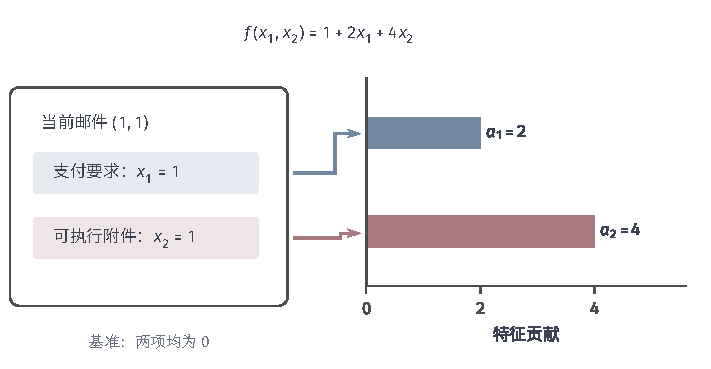
\includegraphics[width=120.407mm]{figures/03-foundations/03-trustworthiness/tikz/trust-feature-attribution/figure.pdf}
  \caption{相对$(0,0)$的教学特征贡献。基准1与当前7相差6，直线路径梯度恒为$(2,4)$，因此IG贡献为2与4。输入标记对应从零起的贡献条，邮件文字只表示规定的二元特征。归因解释分数差，未给出概率或现实因果结论。}
  \label{fig:trust-feature-attribution}
\end{figure*}

\BookSectionRef{sec:game-shapley-order}{第一卷“多方策略的响应与演化”章的“Shapley值”一节}给出了Shapley的一般分配规则。预测解释将联盟价值具体定义为保留特征子集的约定输出。设$N=\{1,\ldots,d\}$，价值为$v(S)$，则
\begin{equation}
 \phi_j=\sum_{S\subseteq N\setminus\{j\}}
 \frac{|S|!(d-|S|-1)!}{d!}
 \bigl[v(S\cup\{j\})-v(S)\bigr]\, .
 \label{eq:interpretability-shapley}
\end{equation}
SHAP（Shapley additive explanations）利用这种分配形成加性贡献。缺失特征怎样补充、使用何种分布，决定$v(S)$及所解释问题\scite{lundberg2017shap}。

边缘背景采样给出$v(S)=\mathbb E[f(\bm x_S,\bm X_{-S})]$，主要比较人工组合上的响应；按已知特征条件采样则保留关联，也可能给未被模型直接读取但预测其他特征的变量分配贡献。二者依定义回答不同问题。精确枚举有指数规模，结构方法或采样近似应报告背景与计算误差。

排列解释可从背景起依次加入当前特征，记录每项加入前后的价值增量，再平均所有进入次序；大量特征时近似采样次序。式~\eqref{eq:interpretability-shapley}正是这种平均。它比较特征组合，IG比较连续路径，二者的共同产物虽是贡献，定义并不相同。

\begin{example}[共同信息的贡献分配]
\label{ex:interpretability-redundancy}
设$v(\varnothing)=0$，$v(\{1\})=v(\{2\})=v(\{1,2\})=1$，任一信息都足够，二者互相替代。每项先进入时增量为1，后进入时为0，Shapley平均得到$1/2$。完整输入中删除一项仍保留价值1，所以分配一半不等于单项移除使输出下降一半。
\end{example}

\paragraph{支持区域的定位}

图像解释可先定位支持目标类别的区域。梯度加权类激活映射（gradient-weighted class activation mapping, Grad-CAM）平均目标分数对卷积特征图的空间梯度，以此给通道加权，并保留正响应。设通道图为$\bm A^k$、空间位置数为$Z$、目标分数为$s_c$，则
\begin{equation}
 \begin{aligned}
 \alpha_k^c&=\frac{1}{Z}\sum_{i,j}
 \frac{\partial s_c}{\partial A^k_{i,j}},\\
 L^c_{i,j}&=\max\!\left(0,\sum_k\alpha_k^c A^k_{i,j}\right)\, .
 \end{aligned}
 \label{eq:interpretability-gradcam}
\end{equation}
梯度表示通道对当前分数的敏感性，特征图给出空间响应，合成结果是粗粒度位置证据。Selvaraju等在多种卷积网络中研究了这种类别定位\scite{selvaraju2017gradcam}。

Grad-CAM定位某层表示中支持类别的区域，IG分配基准分数差。前者受层分辨率、通道梯度平均和正值截断限制，会遗漏反对证据及通道内差异。上采样边缘不能支持像素因果主张，应比较不同类别和对照区域，而非仅凭视觉像物体判断解释质量。

\subsection{基于推理计算过程的解释}
\label{sec:interpretability-local-mechanism}

输入响应提出哪些信息有关，内部解释则固定参数并检验表示、组件和通路怎样参与计算。能从激活解码信息只说明表示含有该信息；替换、屏蔽或恢复后观察行为，才检查计算作用。内部干预也可能制造异常状态，需设置匹配对照。

一种方法先保存干净运行，再构造使目标行为受损的输入，将某位置的干净激活放入受损运行。恢复输出支持该位置在当前设置中的作用。Meng等的因果追踪使用此类实验定位事实关联，并以参数编辑继续检验假设；激活可能携带多因素，其他通路也可能冗余保存，局部恢复不能证明唯一存储\scite{meng2022rome}。

实际实验分别记录干净、受损与单位置替换后的分数$s_{\mathrm{clean}}$、$s_{\mathrm{corrupt}}$和$s_{\mathrm{patch}}$。前者大于受损分数时，可把恢复差相对原差归一化为
\begin{equation}
 r_{\mathrm{restore}}
 =\frac{s_{\mathrm{patch}}-s_{\mathrm{corrupt}}}
        {s_{\mathrm{clean}}-s_{\mathrm{corrupt}}}\, ,
 \label{eq:interpretability-restoration}
\end{equation}
教学值4、0、3给出0.75，表示此次替换恢复四分之三分数差，不能解释为知识量。比例可负或超出1，小分母也会使其不稳。位置恢复图还应在其他输入配对和对照替换中复测。

图~\ref{fig:activation-patching}对应三次运行。在同一计算位置复制激活改变受损分支的后续输出，所有运行使用固定参数。

\begin{figure*}[htbp]
  \centering
  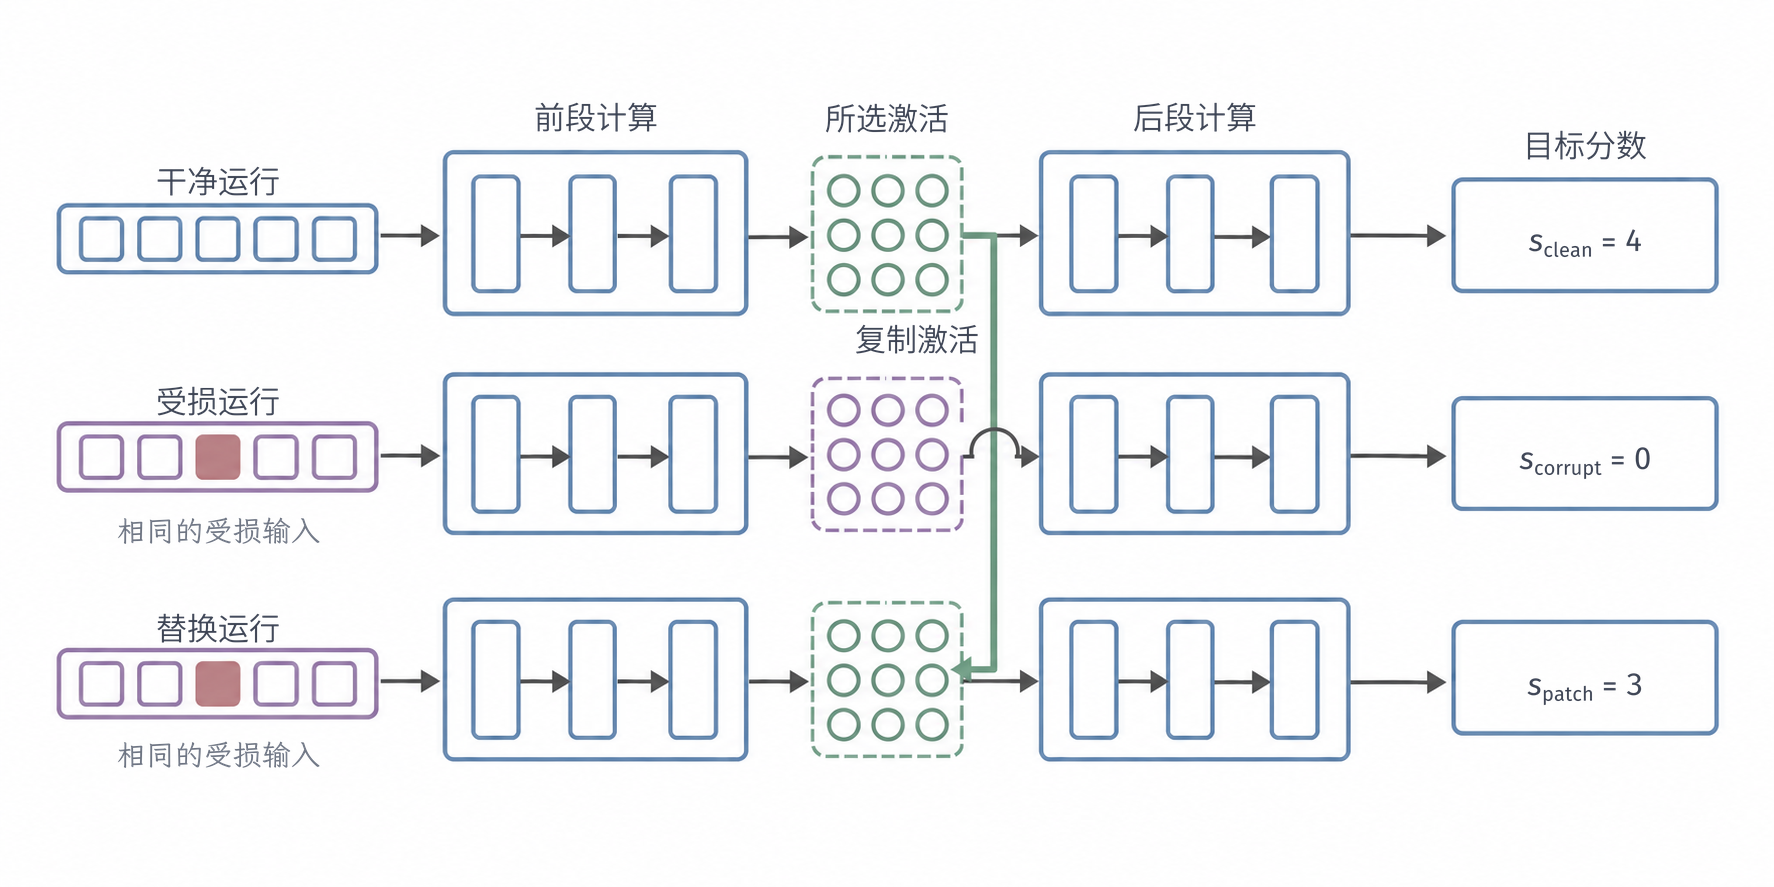
\includegraphics[width=164.600mm]{figures/03-foundations/03-trustworthiness/generated/activation-patching/figure.png}
  \caption{固定参数下的激活恢复试验。第三行保留第二行的受损输入，将干净运行的激活复制到同层同位置后继续前向；教学分数4、0、3给出恢复比例0.75。比例只描述此次分数恢复，不能计量知识或证明唯一位置。绿色复制线与第二行灰色计算线在跨线处不相连。}
  \label{fig:activation-patching}
\end{figure*}

输入归因分配输入作用，机制干预检查内部计算改变后的行为。两者都可能访问激活或梯度，划分依据是主张对象：Grad-CAM主要交付区域定位，激活替换交付内部操作的结果。归因提出的机制假设还需要干预检验，不能直接等同于机制结论。

移除组件后行为消失支持当前设置中的必要性，局部恢复则支持特定背景中的恢复作用。输入污染、替换位置与评分目标都限定结论。多配对、等强度随机替换与组合消融可以排除部分替代解释，单次恢复仍不足以重建全部计算。

工具调用与长生成把解释单位扩展为状态和动作序列。先确定最终行为指标，再定位引入证据的步骤，替换或屏蔽该状态后重放后续过程，检查任务结果。序列干预仍以运行条件为范围；最终文本可能隐藏中间动作的错误。

\subsection{基于训练数据的解释}
\label{sec:interpretability-local-training}

怀疑误拦来自错标训练样本时，需要固定当前邮件，改变训练输入、标签或权重，研究学习后预测的变化。此前的输入和内部解释固定参数，这里则追溯学习怎样产生参数。因此训练样本影响与当前邮件删词效果属于不同实验。

删样本重训练可作直接参照，但成本较高。\term{影响函数}（influence function）利用局部最优解对样本权重的导数近似变化。为固定归一化尺度，先设无另行缩放正则项的平均目标为
\[
 \hat R(\bm{\theta})=\frac1n\sum_{i=1}^n\ell(z_i,\bm{\theta}),
 \qquad
 \bm H=\nabla_{\bm{\theta}}^2\hat R(\hat{\bm{\theta}})\, ,
\]
其中$\hat{\bm\theta}$是局部最优解，$\bm H$可逆，且各损失在当前解的邻域内二阶连续可微。将目标改为$\hat R(\bm\theta)+\epsilon\ell(z,\bm\theta)$，沿附近平稳点分支$\hat{\bm\theta}_\epsilon$对一阶条件求导，得到
\[
 \left.\frac{\mathrm d\hat{\bm{\theta}}_\epsilon}
 {\mathrm d\epsilon}\right|_{\epsilon=0}
 =-\bm H^{-1}\nabla_{\bm{\theta}}
       \ell(z,\hat{\bm{\theta}})\, .
\]
取$z=z_i$时，按$n-1$归一化的删样本目标与$\hat R-\ell(z,\bm\theta)/n$只差正常数倍，具有相同极小点。因此以$\epsilon=-1/n$作一阶外推，有
\[
 \hat{\bm{\theta}}_{-z}-\hat{\bm{\theta}}
 \approx\frac1n\bm H^{-1}\nabla_{\bm{\theta}}
 \ell(z,\hat{\bm{\theta}})\, .
\]
有限外推依赖局部解、光滑性和目标缩放；有正则项时应重推尺度。样本少、单点影响强、解不唯一或训练路径变化都会破坏近似。Koh与Liang研究了该方法的预测追溯应用，实际数据归因还需部分重训练或受控修改复核\scite{koh2017influence}。

对测试样本$z_*$的损失再作一阶展开，删样本效果为
\[
 \ell(z_*,\hat{\bm{\theta}}_{-z})
 -\ell(z_*,\hat{\bm{\theta}})
 \approx\frac1n\nabla_{\bm\theta}\ell(z_*,\hat{\bm\theta})^\top
 \bm H^{-1}\nabla_{\bm\theta}\ell(z,\hat{\bm\theta})\, .
\]
内积取负号对应增加样本权重时的局部变化。这个量由梯度作用定义，不是输入距离：相似邮件可以有不同梯度，不相似错标也可改变边界。大型模型可通过海森向量积近似解线性系统，但计算方式并不消除局部最优前提。

未达到稳定最优时，可用TracIn追踪训练更新的作用。单样本梯度下降中，测试损失下降的一阶近似为
\[
 \ell(z_*,\bm\theta^{(t)})-\ell(z_*,\bm\theta^{(t+1)})
 \approx\eta_t
 \nabla\ell(z_*,\bm\theta^{(t)})^\top
 \nabla\ell(z_i,\bm\theta^{(t)})\, .
\]
$\eta_t$为学习率，梯度针对参数。Pruthi等在保存检查点上累积此类内积，估计哪些样本有助于降低或增加损失。它避免最终海森求逆，但依赖检查点、步长、批处理及优化器，也不等同于从头删样本训练的反事实\scite{pruthi2020tracin}。

\section{解释的质量}
\label{sec:interpretability-quality}

理解线索是否支持主张，需要分别检查五个方面：与模型行为的符合程度，数值与行为范围的覆盖，合理重复下的稳定，读者的正确理解，以及实际使用收益。它们对应保真度、完整性与覆盖、稳定性、可理解性和使用有效性，应独立取证，不能无条件合成通用分数。

验收先固定版本、输出、范围、基准或干预、使用者及用途，再预设指标、比较对象、容忍误差、样本和重复范围、不确定性报告及失败处理。不同论断需要不同实验，例如删除曲线不能统一验证整体规则与训练影响。以下检查按解释对象选择，阈值由用途决定。

图~\ref{fig:trust-explanation-quality-radar}只展示两套教学方案在保真度、覆盖和稳定性上纳入的检查项数。它提示证据缺口；人员理解与使用收益仍需另外检验。

\begin{figure}[!htb]
  \centering
  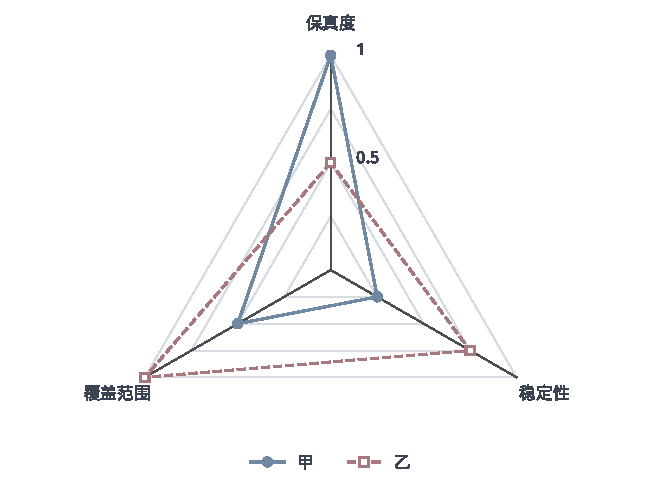
\includegraphics[width=\linewidth]{figures/03-foundations/03-trustworthiness/matplotlib/trust-explanation-quality-radar/figure.pdf}
  \caption{两套构造方案纳入的检查项数。三个维度各预设四项，甲纳入4、2、1项，乙纳入2、4、3项，径向值为项数除以4，线型和标记区分方案。真实检查需预先说明内容与难度；图中面积不合成质量评分，另两项人员与使用评价仍须执行。}
  \label{fig:trust-explanation-quality-radar}
\end{figure}

\subsection{保真度}
\label{sec:interpretability-quality-fidelity}

\term{保真度}（fidelity）度量解释与其声称描述的模型行为是否一致。错误模型也可得到如实解释，因此要与预测正确率分别报告；它也不同于因果图中的faithfulness条件。

案例解释先核查距离和输出是否满足检索定义，再确认案例是否参与预测。邻居投票或原型权重可以重算；事后检索若声称共同因素是依据，则需改变因素检验响应。案例相似本身只验证了检索结果。

反事实需要通过完整系统复算目标结果，报告距离、修改数和有效性条件。声称某项不可缺少时，可撤销该项并比较组合；还应寻找其他近似方案以检查选择偏向。现实可执行性属于行动补救检验，预测翻转只回答模型条件。

代理验收在独立查询样本上比较$f$与$g$。对非负权重$w_i$，标量分数可采用
\[
 \widehat E_{\mathrm{fid}}
 =\frac{\sum_i w_i\,[f(\bm{x}_i)-g(\bm{x}_i)]^2}
        {\sum_i w_i},\qquad \sum_iw_i>0\, .
\]
整体权重应对应参考范围，局部权重对应邻域。类别复述用一致率，概率复述还需分数误差；应按业务分组检查被均值掩盖的分支。交付容限预先设定，独立样本中报告区间或重采样波动，超限时收窄范围或拒绝交付。

归因定义的一致性与干预预测应分开验收。IG检查贡献和，SHAP检查背景与缺失规则；若进一步主张高贡献因素更关键，可按排序逐步删除并与随机、低贡献优先对照，也可从基准逐步插入。曲线和面积支持相应扰动规则下的效果，分配公理不保证在所有删除规则下最优。

扰动实验应匹配改动量与替换方式，并检查输入有效性。删词改变语义、遮挡产生异常块都可能混淆结果。支持与反对证据需分别检查，移除负证据后分数提高有时正符合归因。整体曲线和概念摘要则可在新参考样本上复算，检验重要差异是否复现。

Adebayo等用参数随机化与标签打乱训练检验显著性图是否依赖学得机制。若预测机制改变后，按预设差异指标解释仍未达到最低变化要求，图可能主要反映边缘或架构先验。这个结果应限定在被测方法与设置，不能泛化为所有显著性方法无效\scite{adebayo2018sanity}。

随机化只排除一类缺陷。机制解释应预测新配对中的内部屏蔽或恢复效果，并使用随机位置和等强度替换；训练影响则应对高、低和随机影响样本重新加权或部分重训，核对方向及大小。检验改变的对象应与解释主张相同。

模型理由也是待验收输出，流畅叙述可能来自事后构造。关键证据改变后行为变化而理由未变，会削弱理由解释当前依据的主张。因此需要连接理由与行为试验，语言清晰度只能验证其表达。

\subsection{完整性与覆盖范围}
\label{sec:interpretability-quality-coverage}

完整性既可指分数差分配，也可指行为范围覆盖。具有加性要求的归因可算
\[
 e_{\mathrm{sum}}
 =\left|f(\bm{x})-f(\bm{x}_0)-\sum_j a_j\right|\, ,
\]
$a_j$为归因，IG用残差检查求积，Shapley需改用所定义$v(\varnothing)$与$v(N)$。Grad-CAM没有相同求和承诺。零残差证明约定数值被分完，仍未覆盖全部内部通路或现实原因。

规则和代理应按语言、任务及重要错误预先分组，报告样本量、误差和能够解释的比例。有弃权时同时报告已解释样本质量与总体覆盖，避免只解释简单样本。公式能在未测区域运行，并不构成该区域的解释证据。

机制覆盖需要在多输入、表达与组合中复测局部假设，量化剩余效应。单位置恢复支持当前实验，扩大为一类行为结论时还要承担新范围的证据要求。

\subsection{解释的稳定性}
\label{sec:interpretability-quality-stability}

稳定性先固定哪些条件应保持，再比较结论是否超过预设波动容限。固定模型、输入、基准与定义，重复邻域、背景和概念方向采样可测算法随机性。归因可报均值和标准差，排序可报秩相关，前$k$项可报交并比；可交换编号或方向应先匹配。

任务规定的等价变换提供另一类测试。平移区域须映回坐标，改写词项须匹配单位；输出不变时模型仍可能改变依据，因此要结合响应分析解释差异。越过边界后的解释变化可能忠实。计算重复、输入迁移和重新训练后的复现应分别报告。

解释也要对应该改变的条件作出反应。随机化模型后不变可能是无关性，不能视为稳定优势；声称仅解释函数的方法，对实现同一函数的系统应给出相容结论。预先规定保持项与变化项，才能排除恒定输出图的伪稳定。

\subsection{可理解性}
\label{sec:interpretability-quality-comprehensibility}

可理解性以目标读者是否正确理解为依据。规则数、深度、非零项和概念熟悉度只是负担代理，短而含糊的规则未必比明确计算更容易理解。

人员实验可要求读者根据解释预测新输入的模型反应、比较条件变化或指出适用范围，记录正确率、时间及误解，并匹配难度、事实与背景。在示例~\ref{ex:interpretability-global-local}的规则中判断$(0,1)$是否隔离，可检查加性计算与阈值理解；主观清楚评分不能替代这种检验。

Doshi-Velez与Kim区分实际应用人员评价、简化任务人员评价和无人参与的替代指标。规则少和归因稀疏便于测量，是否对应实际理解仍需人员任务的证据\scite{doshivelez2017rigorous}。

让人预测模型是否拦截，检验对模型的理解；让人判断邮件应否拦截，则同时涉及任务判断能力。实际纠错和错误采纳在下一节评价。喜欢程度只反映主观感受，三者应使用不同观察。

解释组与对照组应获得相同必要事实，否则收益可能来自附加信息。可以保持事实不变只改变组织，或另做附加事实对照。开发者与收件人的背景和任务不同，合适的解释粒度应分别验证。

\subsection{使用有效性}
\label{sec:interpretability-quality-utility}

使用有效性检验解释是否帮助发现错误、减少错误采纳或选择复核，并考虑时间和认知成本。理解模型只是前提，实际结果仍须在接近真实的决策任务中评价；补救执行效果另见第~\ref{sec:interpretability-recourse-validation}节。

可比较无解释、所提解释与等信息量说明，匹配任务难度并记录最终损失、纠错、错误否决和用时。题目随机分配或顺序平衡减少记忆影响。模型错误建议的采纳率应单列，整体采纳增加也可能来自过度信任。

教学例中，两组各处理100封匹配邮件，模型均错20次。解释组纠正15次却新增8错，对照组纠正10次但只新增1错，最终分别为$20-15+8=13$与$20-10+1=11$。纠错更多并未使最终错误更少；实际比较还需足够样本估计差异不确定性。

保真、覆盖、稳定、理解与收益构成不同证据链，前项成立不自动推出后项。简化导致的取舍应指出具体维度和输入范围。交付解释还应明确接收者与需要完成的判断或行动。

\section{行动补救}
\label{sec:interpretability-recourse}

误拦解释之后，使用者还需要可执行恢复路径。\hyperref[sec:interpretability-local-counterfactual]{“不同结果的反事实比较”段}找到了改变判断的输入，尚未说明如何实现。\BookSectionRef{sec:causal-action-recourse}{第一卷“因果响应”章的“行动补救”一节}定义了\term{行动补救}（algorithmic recourse）、可行行动与后果模型；这里进一步考察权限、流程负担、公平与现实验证。

补救依次确定行动和目标、在约束中比较方案、核验执行与结果。行动后果决定是否有解，成本决定如何选择，现实验证决定模型中的可行结论能否落实。以下沿同一方案展开这三个环节。

\subsection{补救行动的确定}
\label{sec:interpretability-recourse-target}

行动范围先由执行者权限确定。发送方可纠正来源记录、补充证明或转换附件，收件人可能只可请求复核，运营方可修正提取错误或调整流程。一方可做的操作不能直接推荐给另一方。

候选路径可从记录纠错、现实条件改变和流程申诉中获得。前两类通常经新输入重新判断，后一类还改变决策流程，应说明处理者、依据与时限。进入人工复核也不是简单降低模型分数。

补救目标应包含真实任务。删除付款要求可能使邮件放行，却也删掉业务请求；目标因此应同时检查恰当处理与内容保留。若期望复核，应检验是否进入并完成流程，而不是强求立即有利分类。

候选行动须列出执行者、对象、资源、时长和预期变化。例如，由发送方把附件转换成保留必要信息且无可执行内容的格式再提交，才构成可实施方案。解释产生线索，领域知识与权限决定线索能否执行。

设当前状态为$\bm x$，行动后果为$T(\bm x,a)$，它描述字段及其他状态随$a$怎样变化。固定决策时结果为$\hat y(T(\bm x,a))$；流程复核则需另定义结果。小输入距离不代表低行动成本，记录改写也未必改变相应事实。

\subsection{补救行动的选择}
\label{sec:interpretability-recourse-action}

行动集合由不可变属性、权限、方向和取值限定，后果又受预算、截止时间与业务内容限制。合同信息必须保留等条件应作为硬约束；可行方案之间的时间或费用偏好进入目标。筛选与排序分别承担这两种作用。

令允许行动集为$A(\bm x)$、成本为$c(a;\bm x)$、目标输出集为$Y_{\mathrm{goal}}$。固定规则下的低成本方案可求
\begin{equation}
 \begin{aligned}
 \min_{a\in A(\bm{x})}\quad &c(a;\bm{x})\\
 \text{满足}\quad &\hat y(T(\bm{x},a))\in Y_{\mathrm{goal}}\, .
 \end{aligned}
 \label{eq:interpretability-recourse}
\end{equation}
$A$规定允许行动，$T$计算后果，输出约束检验达标，$c$比较达标方案。目标约束下存在可行行动才有补救，最优性则还依赖所声明范围、后果和成本，不能脱离这些条件推广。

成本要对应实际负担。时间、费用和次数可以分列，合成时需解释权重。一个方案各项成本不高于另一个且至少一项更低时，前者支配后者；存在不同偏好时可提供不被支配方案供选择。资源约束变化也可能改变最优方案。

Ustun等将可行动变量、变化方向、离散值和成本写入线性分类器的整数规划，搜索达到目标的行动，并分析哪些个体缺少方案。这使输入翻转落实为明确的行动约束问题\scite{ustun2019recourse}。

少量候选可枚举后果与成本，连续离散混合行动可在适用模型下规划或搜索。发现可行解证明存在，有限搜索失败不证明无解；全局最优需要完备搜索或有效最优性界，否则应声明当前搜索范围。

行动后果往往相互依赖。培训提升技能也占用时间，可能降低当期资源，不能在输入表中独立设定。Karimi等利用结构因果模型计算干预沿后继变量的影响，再在行动空间优化成本\scite{karimi2021interventions}。

\begin{example}[约束与成本决定补救方案]
\label{ex:interpretability-causal-recourse}
教学申请规则在$s+r\geq3$时批准，$s$为技能分数、$r$为当期资源，当前$(1,1)$被拒。直接把技能记录改为2可以翻转模型，但培训$a\geq0$实际造成$s'=1+a$、$r'=1-a/2$，总分为$2+a/2$，需$a\geq2$。如果培训上限为1，仅培训就无法达标。

在上述培训上限为1的条件下，再允许资源支持$0\leq b\leq1$，令$r'=1-a/2+b$，组合成本为$c(a,b)=a+3b$。目标要求$a/2+b\geq1$；单独支持$(0,1)$成本3，组合$(1,1/2)$成本2.5，二者均达标。

在这些条件下，可行解满足$b\geq1-a/2$，所以$c\geq3-a/2\geq2.5$，组合$(1,1/2)$达到下界而最优。预算改为2时，所有允许组合的最低成本仍高于预算，因而无解。这个无解结论来自后果方程和成本下界，而非搜索失败。
\end{example}

图~\ref{fig:trust-actionable-recourse}比较记录改动与行动路径。行动可行性同时依赖权限、后果与预算，模型翻转只是其中一项条件。

\begin{figure}[htbp]
  \centering
  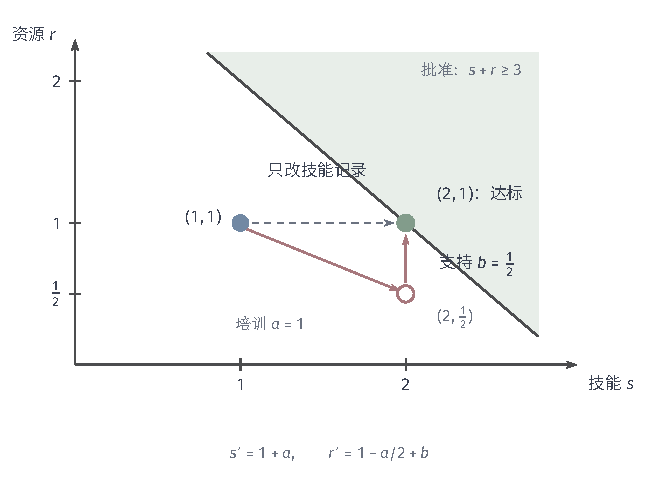
\includegraphics[width=\linewidth]{figures/03-foundations/03-trustworthiness/tikz/trust-actionable-recourse/figure.pdf}
  \caption{示例~\ref{ex:interpretability-causal-recourse}的约束补救组合。虚线表示只改技能记录；培训$a=1$实际先到$(2,1/2)$，支持$b=1/2$再到批准边界。仅培训且上限为1无法达标，组合成本2.5；预算为2时，成本下界证明允许集合中无可行方案。}
  \label{fig:trust-actionable-recourse}
\end{figure}

后果或未来模型不确定时，可要求候选在一组有依据情形中均达标，或在明确概率模型中达到预设成功率。容限取自任务风险，要求收紧可能增加成本或导致无解。无解应定位预算、权限、后果或规则的限制，再考虑复核及流程调整。

模型内可算还不同于证据可识别。多套结构模型可能符合相同观察甚至边缘干预资料，却预测不同个体后果。应先声明证据与领域假设允许的模型类，再报告方案、成本与成功概率对模型的敏感性，必要时施加类上的稳健约束。第一卷条件反事实的识别边界仍适用，缺失识别依据不能仅当参数误差处理。

\subsection{补救效果的验证}
\label{sec:interpretability-recourse-validation}

补救验收分为计算与执行两层：前者核对约束和目标，后者比较真实后果。第~\ref{sec:interpretability-quality-utility}节检查解释怎样影响人的判断，这里检查行动实施后的结果，满意度不能同时替代两种证据。

\paragraph{方案与约束的复核}

对方案重查权限、不可变属性、取值、时限与预算，再由$T$产生状态，通过实际特征处理和决策重算。代理或连续近似得出的候选须回到真实系统验证。成本最优性可用穷举、精确小问题或有效求解界复核，无法证明时另报限制。

在示例~\ref{ex:interpretability-causal-recourse}中，代入教学组合$(1,1/2)$得到$(s',r')=(2,1)$、总分3、成本2.5，并满足行动上限，证明模型内可行达标；成本下界另证最优。若预算为2，该达标候选仍不可执行。

\paragraph{行动后果与实际收益的检验}

实际记录应包含行动完成、费用、状态变化与最终目标。将新状态与$T$预测对照，才能发现后果高估。技能与资源的观察相关通常不足以预测个人培训效果，可结合干预证据、对照研究与执行记录检验假设，并限定支持范围。

若实际培训每单位消耗资源0.8，组合$(1,1/2)$后状态为$(2,0.7)$，总分2.7而未达标。计算仍符合所设模型，失效来自后果假设。修订应重估后果并重新求方案，不能引用原最优性证明现实有效。

方法评价应分别报告建议可行、实际完成和完成后达标的比例，以及费用和不利后果，并明确每项分母。仅统计执行成功者会遗漏无方案与无法执行者。按群体报告无解、完成、成功、等待和成本分布，可检查不可接受属性路径及申诉负担；个体可行性与制度公平不同，口径见第~\ref{chap:trust-fairness}章。声称建议产生收益时，还需与无建议或既有方式对照，处理自选择差异。

验收还应核对业务目标。邮件放行但合同损坏、评分下降但实际风险仍在，都未完成补救。复核与申诉要观察实质处理、错误纠正和时间负担，分别报告决策变化与真实收益。

\paragraph{效果保持与失效处理}

行动需要时间，因此应标明模型版本、后果假设和有效条件。周期较长时，更新或环境变化可能使方案失效，可在有依据的情形中重算或跟踪实施结果；有限情形不能保证所有未来条件。

无法完成操作时修订行动集，实际后果不符时修订$T$，规则或流程变化时重查目标。候选、约束优化和验证据此形成修订循环。仍无可行方案的个体，应得到明确限制和可用复核途径。

\section{本章小结}
\label{sec:interpretability-summary}

章首三个问题对应不同解释范围。整体规则描述一组邮件的判断，单次证据定位当前拦截；结构、输入和语义分别交代计算组合、具体因素作用及对应含义。结合使用时仍需明确每项主张的范围。

单次解释可以围绕输入响应、内部计算或学习经历取证。案例、反事实、代理和归因固定模型，内部干预改变运行，训练追溯改变学习。贡献可复算不等于机制已确定，内部通路也不等于现实因果；把局部结果汇总为整体结论，还须检验异质性与覆盖。

解释的五类质量分别对应模型、范围、重复、读者和使用任务。补救还需行动权限、后果模型及识别依据，并核查群体机会和成本。清晰解释仍可能如实揭示错误或不公平依赖；展示训练经验和私人特征也会引入披露问题。下一章据此讨论数据、模型发布和信息公开中的隐私保护。

\paragraph{延伸阅读}

Doshi-Velez与Kim的框架可用于区分人员实验和替代指标；LIME与积分梯度则适合比较邻域代理和基准贡献所支持的不同主张。阅读时沿评价对象与证据条件分析，而非仅比较可视化外观\scite{doshivelez2017rigorous,ribeiro2016lime,sundararajan2017ig}。

反事实解释与因果补救可对照阅读。Wachter等搜索邻近目标输入，Karimi等加入行动及连带后果；两条路线分别验证预测条件与行动方案，其差别来自待优化对象\scite{wachter2018counterfactual,karimi2021interventions}。
